\section{Experiments}
\label{sec:experiments}

Our experimental analysis addresses four questions:
(1) How does CORELS' accuracy compare to other algorithms?
(2) How rapidly does the objective function converge?
(3) How rapidly does CORELS prune the search space?
(4) How much does each of the implementation optimizations contribute to CORELS' performance?
All results presented use the COMPAS data set unless otherwise noted,
and were executed on (describe machine) \dots
[Sentence that we have more experiments]

We first ran a 10-fold cross validation experiment using CORELS and eight other algorithms:
GLM, SVM, AdaBoost, CART, C4.5, RF, RIPPER, and scalable rule lists (SBRL).
There were no statistically significant differences in the accuracies of the
algorithms. In fact, the difference between folds was far larger than the difference
between algorithms. We conclude that CORELS produces models whose accuracy is comparable
to those found via other algorithms.

Figure \ref{fig:objective} illustrates how both the objective and the size of
the remaining search space decrease as CORELS executes.
The objective drops quickly, achieving the optimal value within 10 seconds.
CORELS certifies optimality in less than 6 minutes --
the objective lower bound of the remaining search space
monotonically converges to the optimal objective
as the search space steadily shrinks.

Finally, we determine the efficacy of each of our data structure and bounding
optimizations.
Table \ref{tab:ablation} provides sumary statistics for experiments using
the full CORELS implementation and implementations with a specific
optimization removed.
Figure \ref{fig:queue} presents a view of the same experiments, focusing
on just three of the optimizations. These charts depict the number of rule
lists of a given length in the queue during the algorithm's execution.


\begin{arxiv}
\begin{table}[t]
\centering
\begin{tabular}{l | c | c}
Method & ProPublica & NYCLU \\
\hline
CORELS & 67.6 $\pm$ 2.0 & 69.8 $\pm$ 2.7 \\
SBRL & 67.1 $\pm$ 1.7 & 69.7 $\pm$ 2.0 \\
CART & 66.7 $\pm$ 2.1 & 69.8 $\pm$ 2.7 \\
C4.5 & 67.3 $\pm$ 1.8 & 66.8 $\pm$ 2.1 \\
RF & 67.3 $\pm$ 1.8 & 68.7 $\pm$ 2.4 \\
RIPPER & 67.3 $\pm$ 2.0 & --- \\
AdaBoost & 67.3 $\pm$ 1.7 & 70.6 $\pm$ 2.7 \\
GLM & 67.5 $\pm$ 1.8 & 70.3 $\pm$ 2.5 \\
SVM & 67.1 $\pm$ 2.0 & 70.2 $\pm$ 2.7 \\
\end{tabular}
\vspace{5mm}
\caption{Comparison with other methods:
Means and standard deviations of test error.
Also report algorithm runtimes (mean $\pm$ standard deviation over 10 folds).
CORELS ${\Reg = 0.005}$ for ProPublica and ${\Reg = 0.01}$ for NYCLU.}
\label{tab:comparison}
\end{table}
\end{arxiv}

\begin{figure}[t!]
\begin{center}
%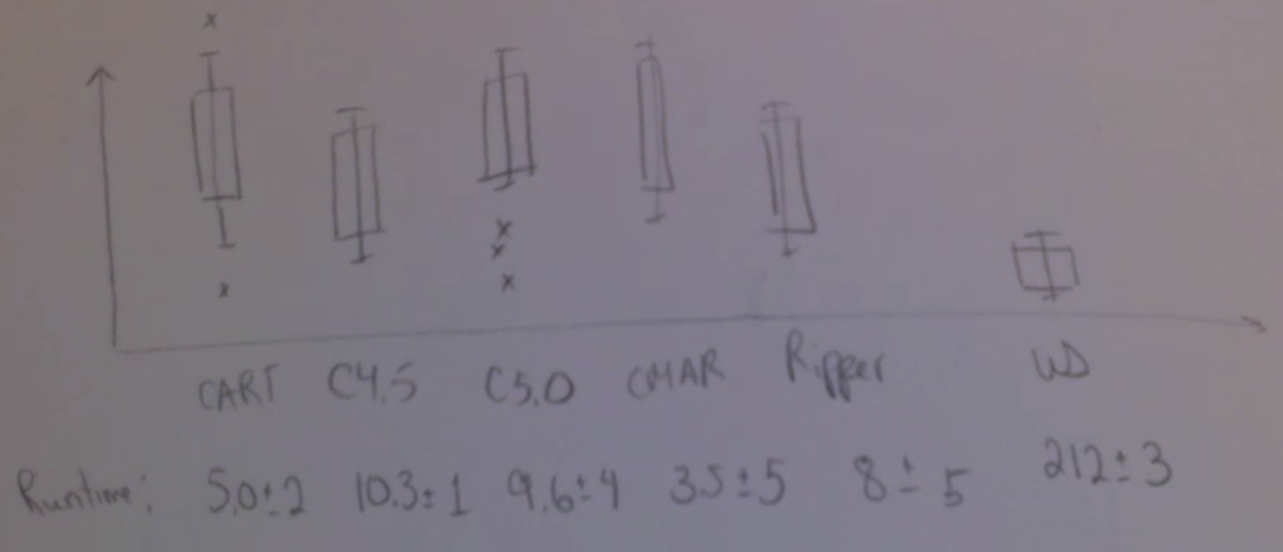
\includegraphics[width=0.75\textwidth]{figs/sketch-comparison.png}
\begin{arxiv}
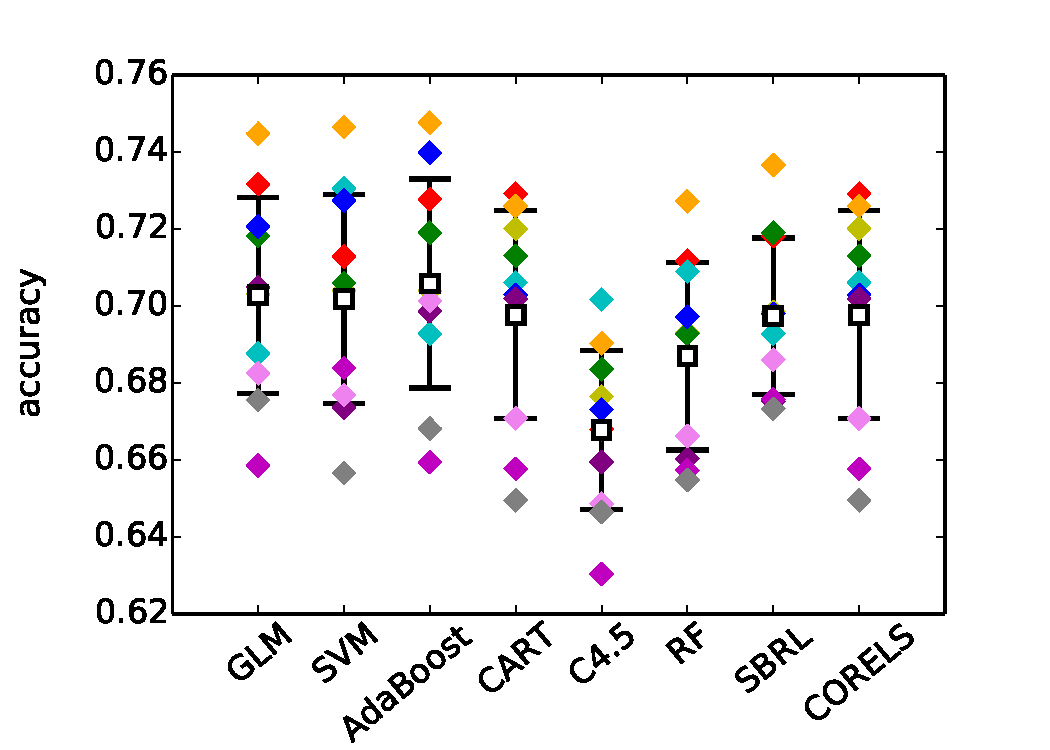
\includegraphics[width=0.75\textwidth]{figs/compare-compas.pdf}
\end{arxiv}
\begin{kdd}
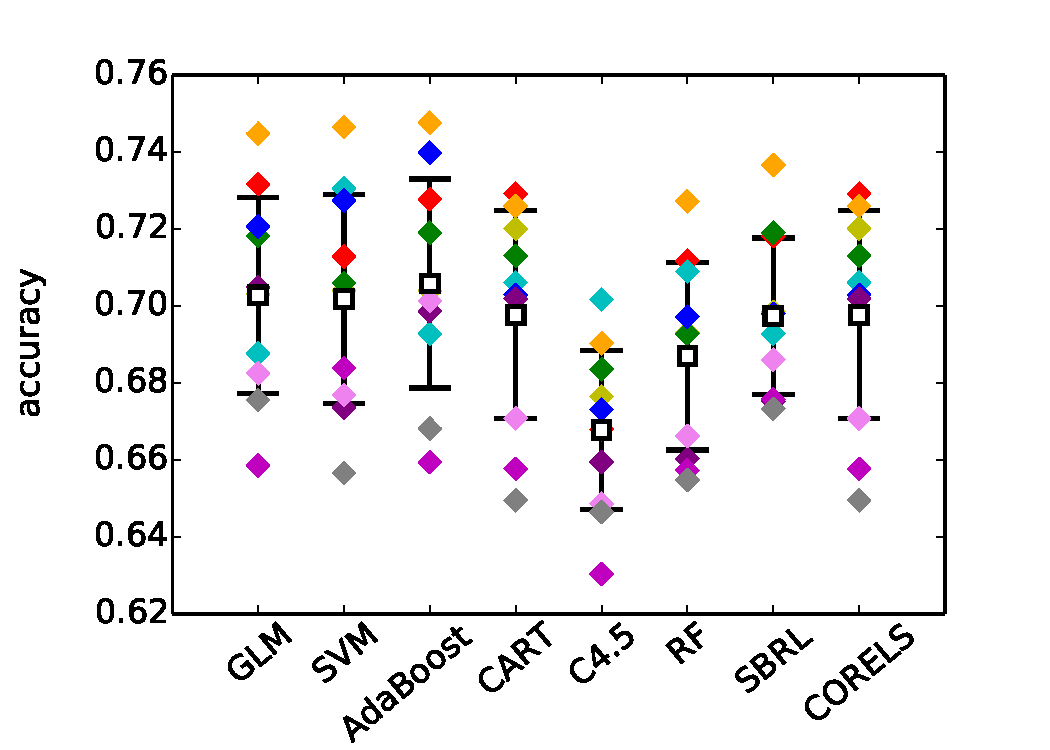
\includegraphics[width=0.4\textwidth]{figs/compare-compas.pdf}
\end{kdd}
\end{center}
\caption{Comparison with other methods:
Test error for us and a few other algorithms
(CART, C4.5, CBA, CMAR/CPAR, C5.0, Ripper, \dots),
as a function of sparsity over 10 folds, for one big dataset (box plots).}
\label{fig:comparison}
\end{figure}

\begin{arxiv}
\begin{figure}[t!]
\begin{center}
\end{center}
\caption{Missing:  Test error as a function of regularization and sparsity
(number of rules) as a function of regularization, over 10 folds,
for one big dataset.}
\label{fig:regularization}
\end{figure}
\end{arxiv}

\begin{arxiv}
\begin{figure}[t!]
\begin{center}
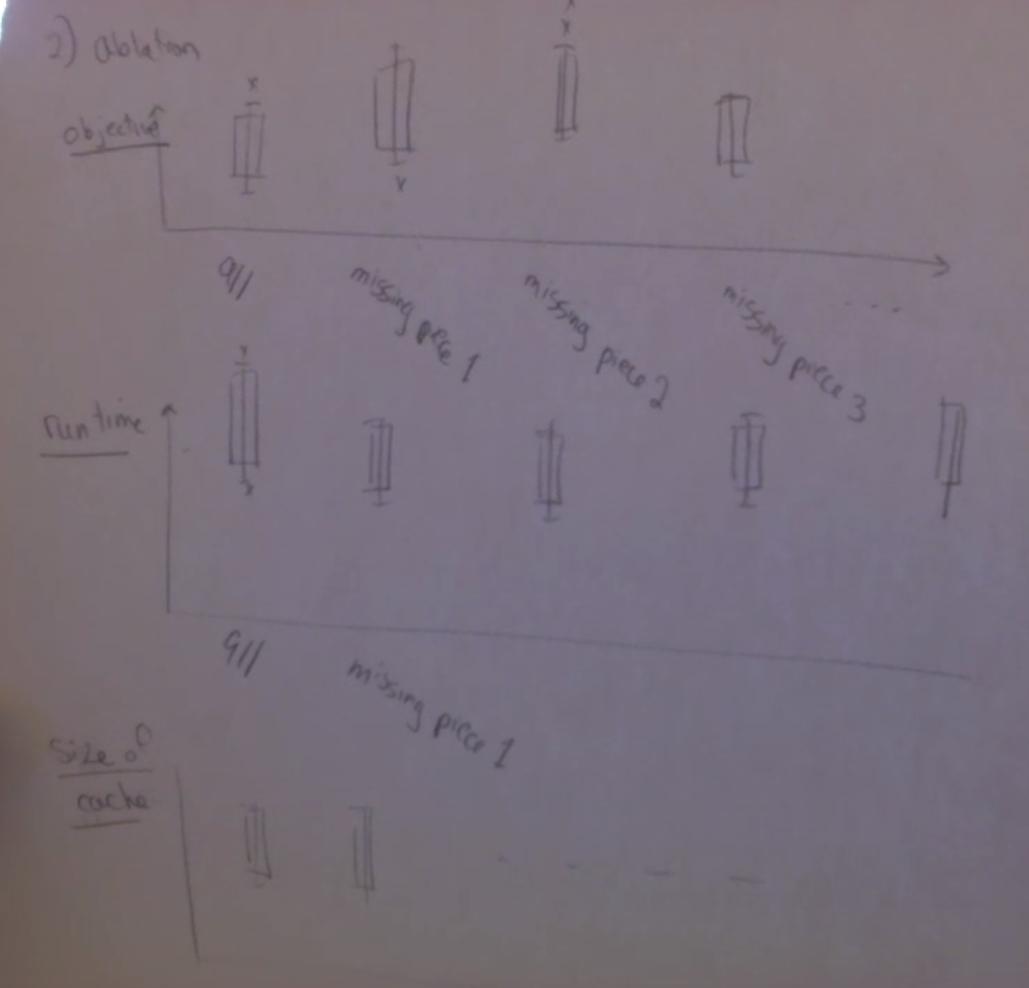
\includegraphics[width=0.75\textwidth]{figs/sketch-ablation.png}
\end{center}
\caption{Ablation experiment:
Show the effect of each ``piece'' at a time,
run X without each in turn and show the difference in either
quality of solution or runtime or amount of memory, size of cache or queue,
where X is a specific implementation
(meaning a specific scheduling policy and node type)}
\label{fig:ablation}
\end{figure}
\end{arxiv}

\begin{arxiv}
\begin{figure}[t!]
\begin{center}
\end{center}
\caption{Missing:  Some sort of comparison of different scheduling policies}
\label{fig:scheduling-policy}
\end{figure}
\end{arxiv}

\begin{arxiv}
\begin{figure}[t!]
\begin{center}
%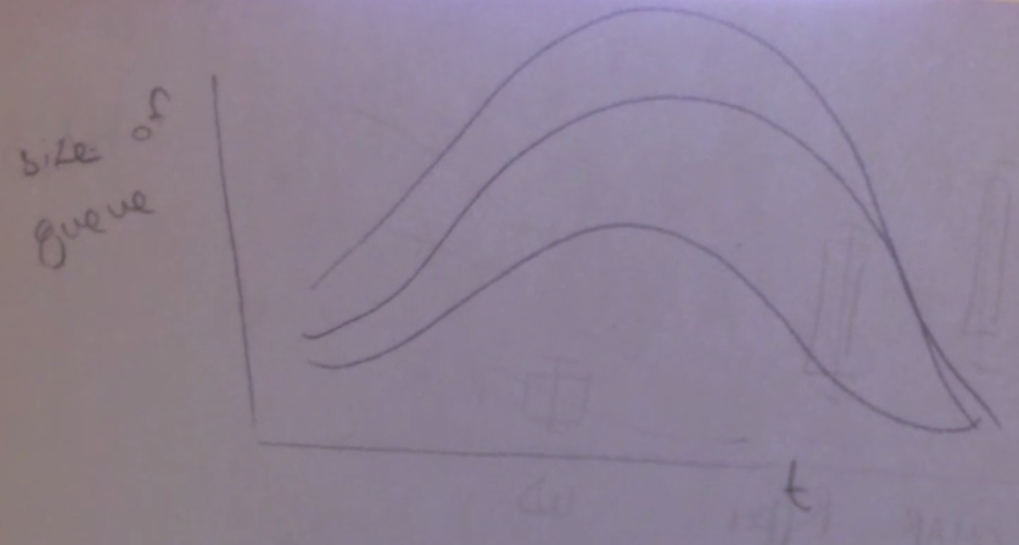
\includegraphics[width=0.65\textwidth]{figs/sketch-queue-size.png}
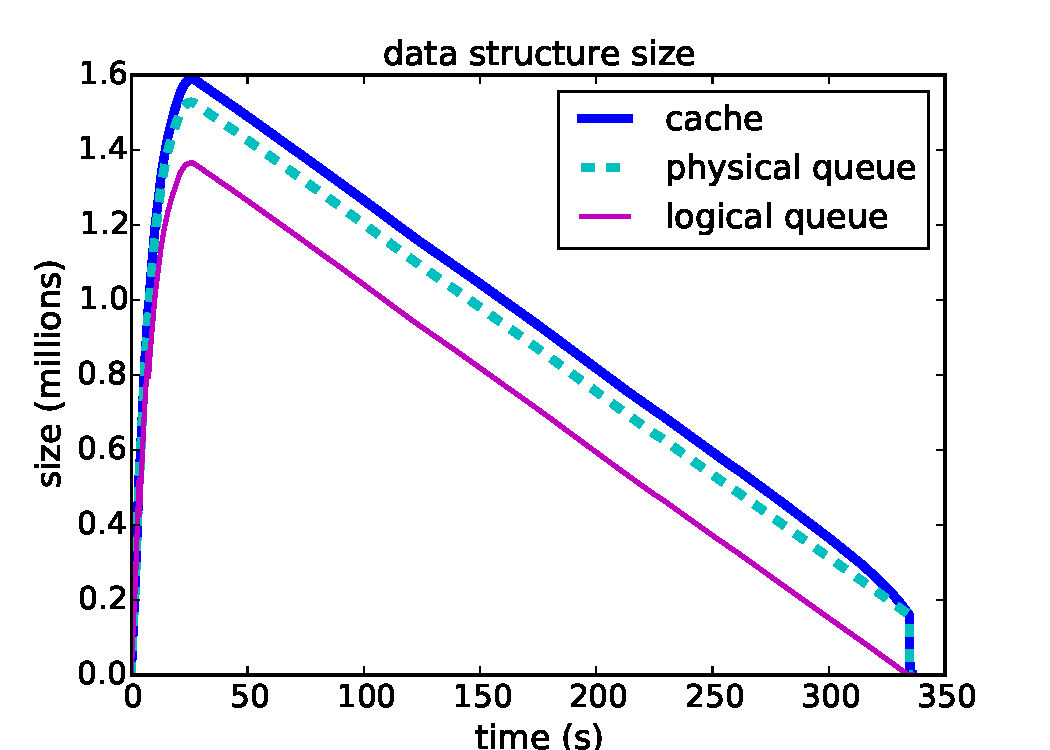
\includegraphics[width=0.8\textwidth]{figs/ela_compas-queue-cache-size-insertions.pdf}
\end{center}
\caption{Cache and queue data structure sizes and insertions.
%
The top plot shows the sizes of the cache and queue data structures,
as a function of wall clock time.
%
The number of nodes in the cache (solid black line) is an
upper bound on the number of elements in the physical queue
(dotted gray line), since the physical queue elements only
correspond to the cache trie data structure's leaf nodes
plus disconnected cache nodes that have been marked for deletion.
%
The queue's physical size is an upper bound on its
logical size (solid blue line), which doesn't include nodes
that have been marked for deletion.
%
The bottom plot shows the cumulative number of cache insertions,
which is equivalent to the cumulative number of queue insertions,
as a function of wall clock time.
}
\label{fig:queue-cache-size-insertions}
\end{figure}
\end{arxiv}

\begin{figure}[t!]
\begin{center}
%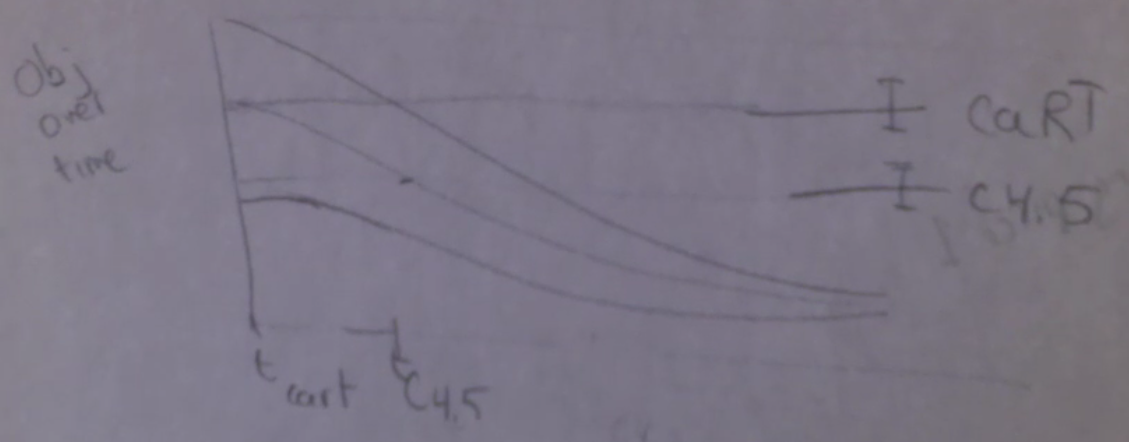
\includegraphics[width=0.65\textwidth]{figs/sketch-objective.png}
\begin{arxiv}
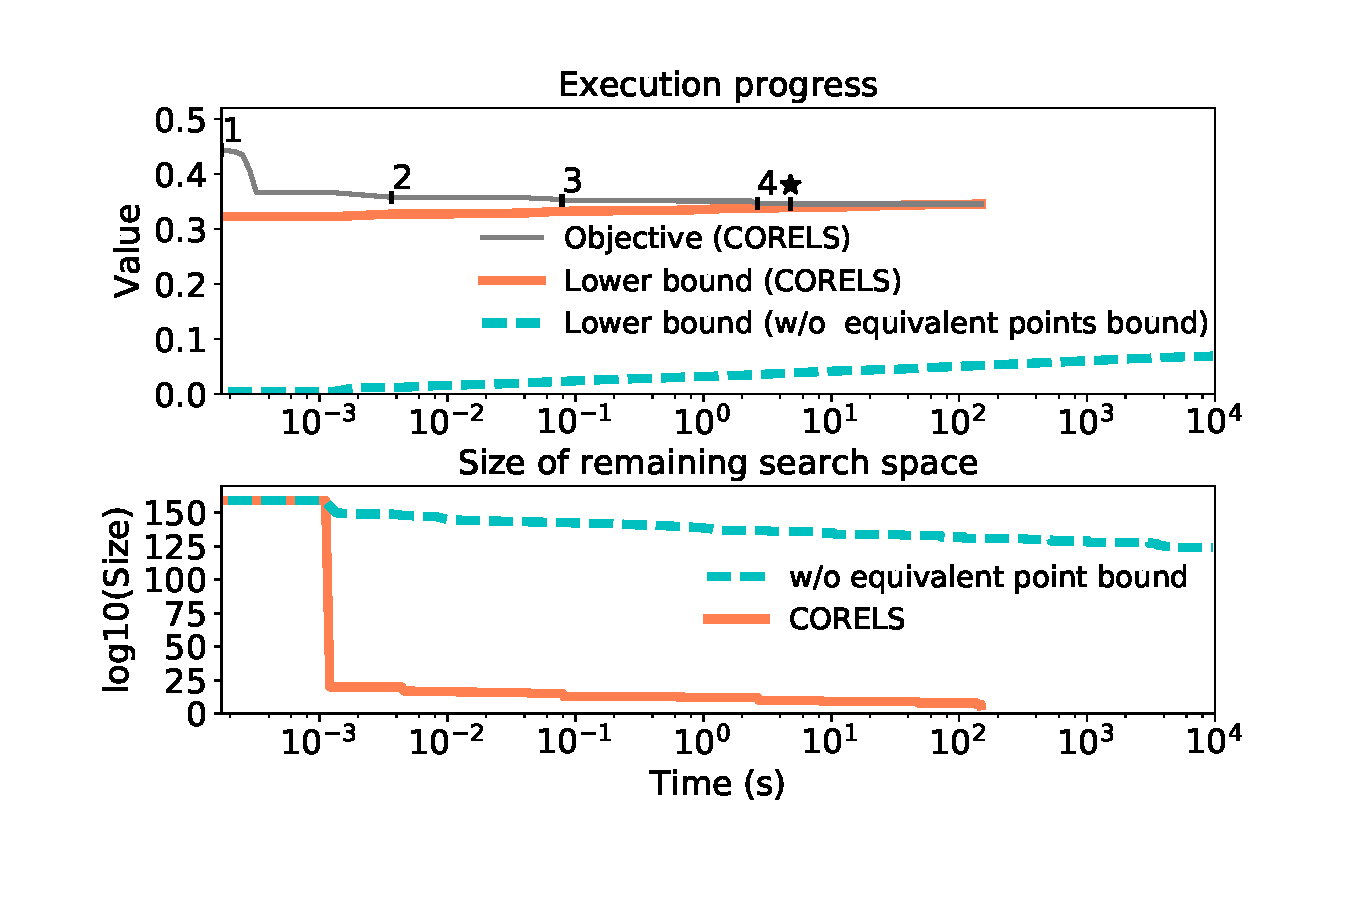
\includegraphics[width=0.8\textwidth]{figs/compas_execution-remaining-space.pdf}
\end{arxiv}
\begin{kdd}
% left lower right upper
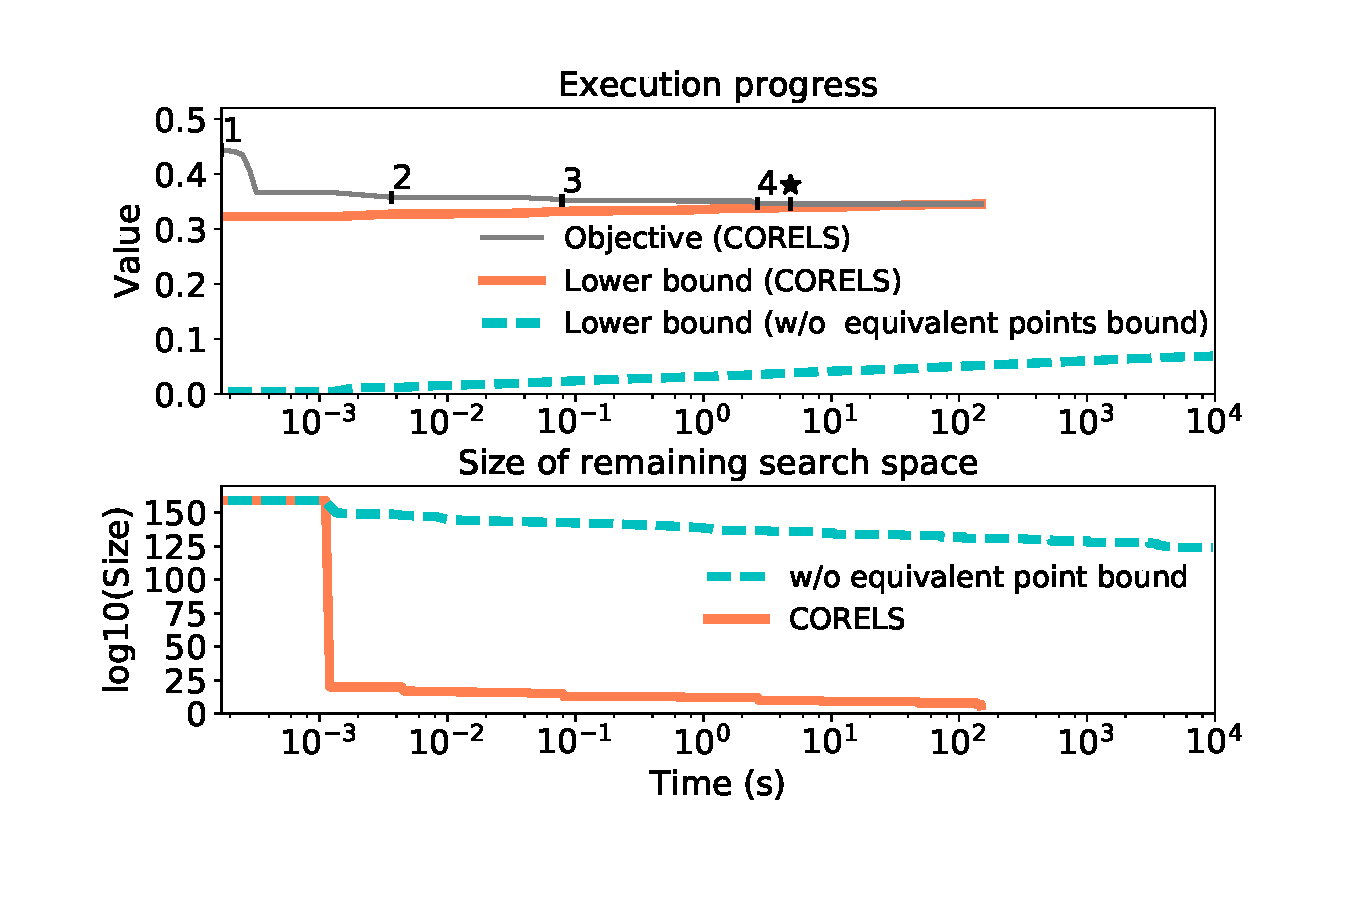
\includegraphics[trim={20mm, 25mm, 10mm, 5mm}, width=0.45\textwidth]{figs/compas_execution-remaining-space.pdf}
\end{kdd}
\end{center}
\caption{Example executions of CORELS with (solid lines) and without
(dashed lines) the equivalent points bound from Theorem~\ref{thm:identical}.
%
Top: Objective value (thin solid line) and lower bound (thick solid line)
for CORELS, as a function of wall clock time (log scale).
%
Numbered hatch marks along the objective indicate when the length of
the best known rule list changes, and are labeled by the new length.
%
CORELS quickly the optimal value (star marker),
and certifies optimality when the lower bound matches the objective value.
%
We also plot the lower bound (dashed line) from a separate execution
of CORELS that does not leverage the equivalent points bound.
%
The large gap between this lower bound and the optimum
demonstrates that this execution is far from complete.
%
%(For clarity, we do not plot the corresponding trace of the objective value.)
%
%Missing: horizontal lines and x-ticks for CART and C4.5.
%
Bottom:
$\lfloor \log_{10} \Remaining(\CurrentObj, \Queue) \rfloor$
as a function of wall clock time,
where~$\Remaining(\CurrentObj, \Queue)$ is the upper bound
from Theorem~\ref{thm:remaining-eval-fine}
on the size of the remaining search space.}
\label{fig:objective}
\end{figure}

\begin{table}[t]
\centering
%\small
\resizebox{0.49\textwidth}{!}{
\begin{tabular}{l | c | c | c | c | c}
Removed & $t_\text{total}$ & $t_\text{opt}$ & $i_\text{total}$ & $Q_\text{max}$ & $K_\text{max}$ \\
component & (min) & (s) & ($\times 10^6$) & ($\times 10^6$) & \\
\hline
none (CORELS) & 5.5 (1.6) & 8 (2) & 1.7 (0.4) & 1.3 (0.4) & 5-6 \\
priority queue & 6.7 (2.2) & 4 (1) & 1.9 (0.6) & 1.5 (0.5) & 5-6 \\
support bounds & 10.2 (3.4) & 13 (4) & 2.7 (0.8) & 2.2 (0.7) & 5-6 \\
permutation map & 58.6 (23.3) & 23 (6) & 16.0 (5.9) & 14.5 (5.7) & 5-6 \\
lookahead bound & 71.9 (23.0) & 9 (2) & 18.5 (5.9) & 16.3 (5.3) & 6-7 \\
%equiv. pts. bound & 188.6 (104.6) & 6178 (1840) & 803.8 (0.1) & 790.5 (0.4) & 10-10
equiv. pts. bound & $>$134 & $>$7168* & $>$800 & $>$789 & $\ge$10
\end{tabular}
}
\vspace{5mm}
\caption{Per-component performance improvement.
%
The columns report the total execution time (minutes),
time to optimum (seconds), number of queue insertions (millions),
maximum queue size (millions), and maximum evaluated prefix length.
%
The first row corresponds to our full CORELS algorithm,
and subsequent rows to variants that each exclude a specific
implementation optimization or bound removed.
%
(We are not measuring the cumulative effects of removing a sequence of components.)
%
All rows represent complete executions, except for the final row,
in which each execution was terminated due to memory constraints,
%once the size of the cache reached ${8 \times 10^8}$ elements,
after consuming 390-410GB RAM.
%
In all but the final row and column, we report averages
(with standard deviations, in parentheses) over 10 cross-validation folds;
in the final row, we report thresholds that reflect minimum values across folds. \\
%
*~Only 4 out of 10 folds achieve the optimum.
}
\label{tab:ablation}
\end{table}

\begin{figure}[t!]
\begin{center}
\begin{arxiv}
%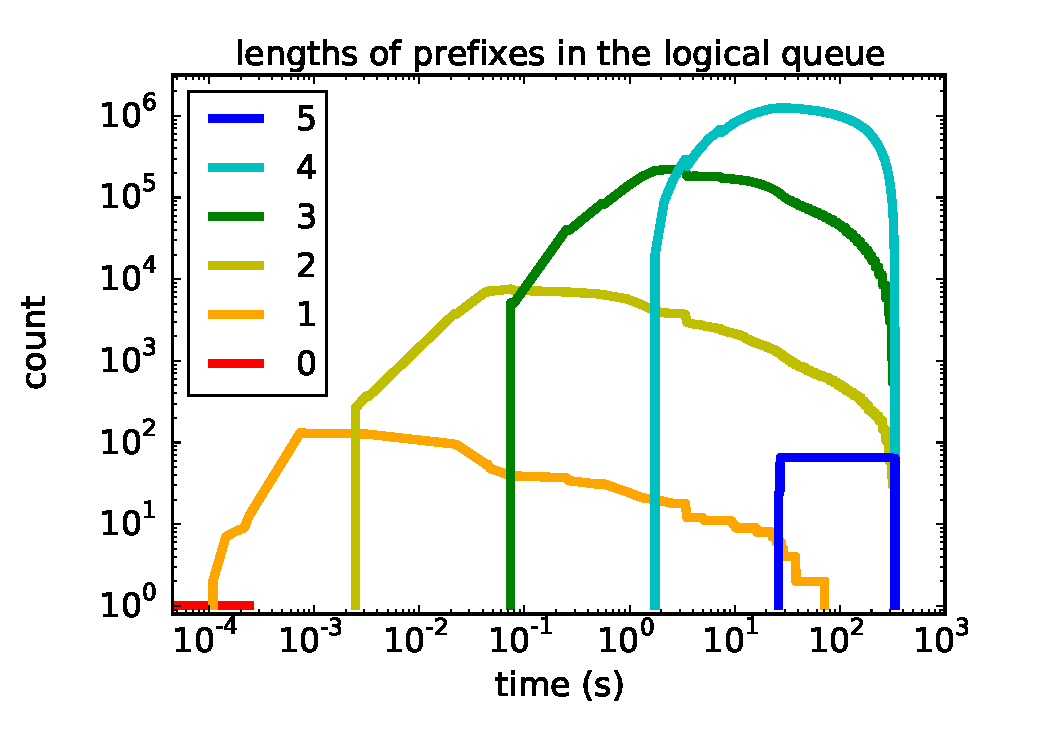
\includegraphics[width=0.8\textwidth]{figs/ela_compas-queue.pdf}
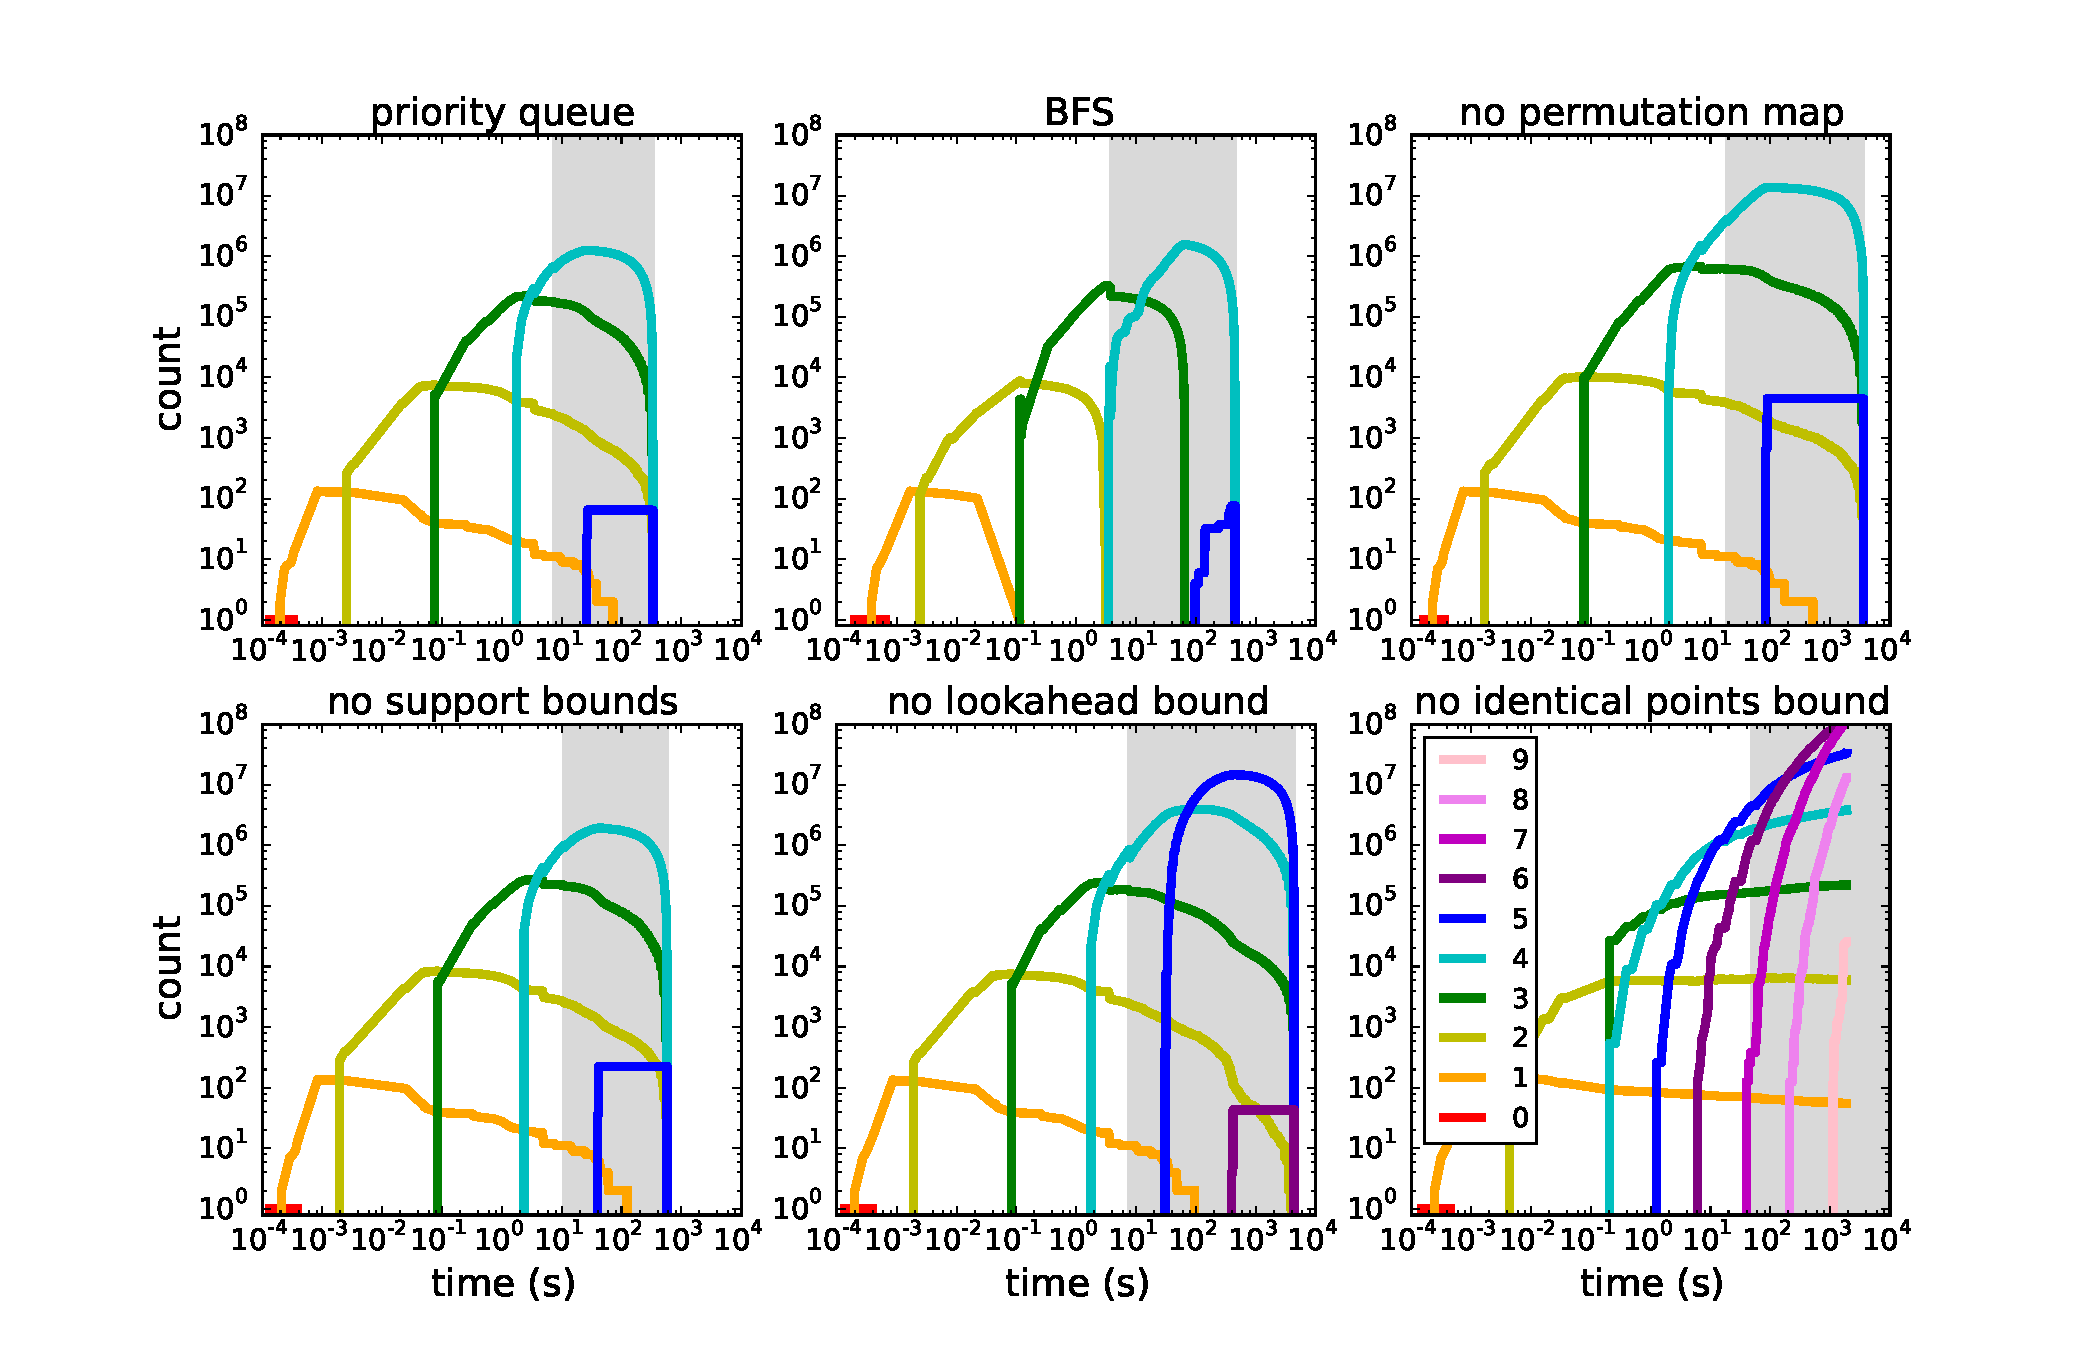
\includegraphics[width=\textwidth]{figs/ela_compas_compare-queue.pdf}
\end{arxiv}
\begin{kdd}
%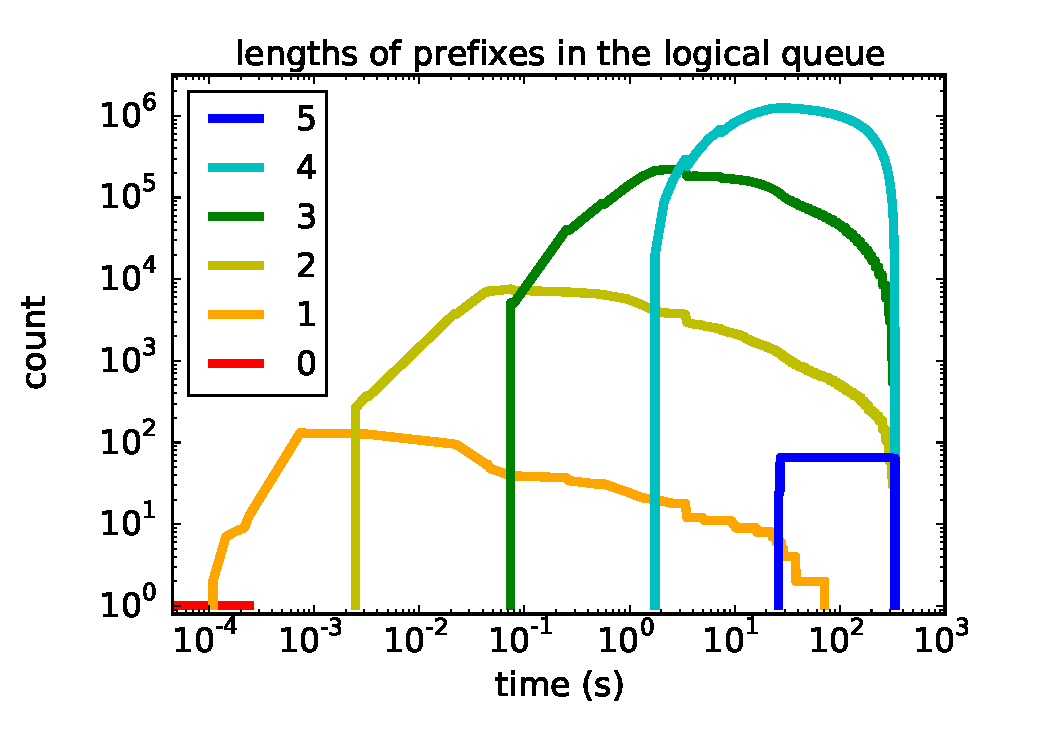
\includegraphics[width=0.5\textwidth]{figs/ela_compas-queue.pdf}
% left lower right upper
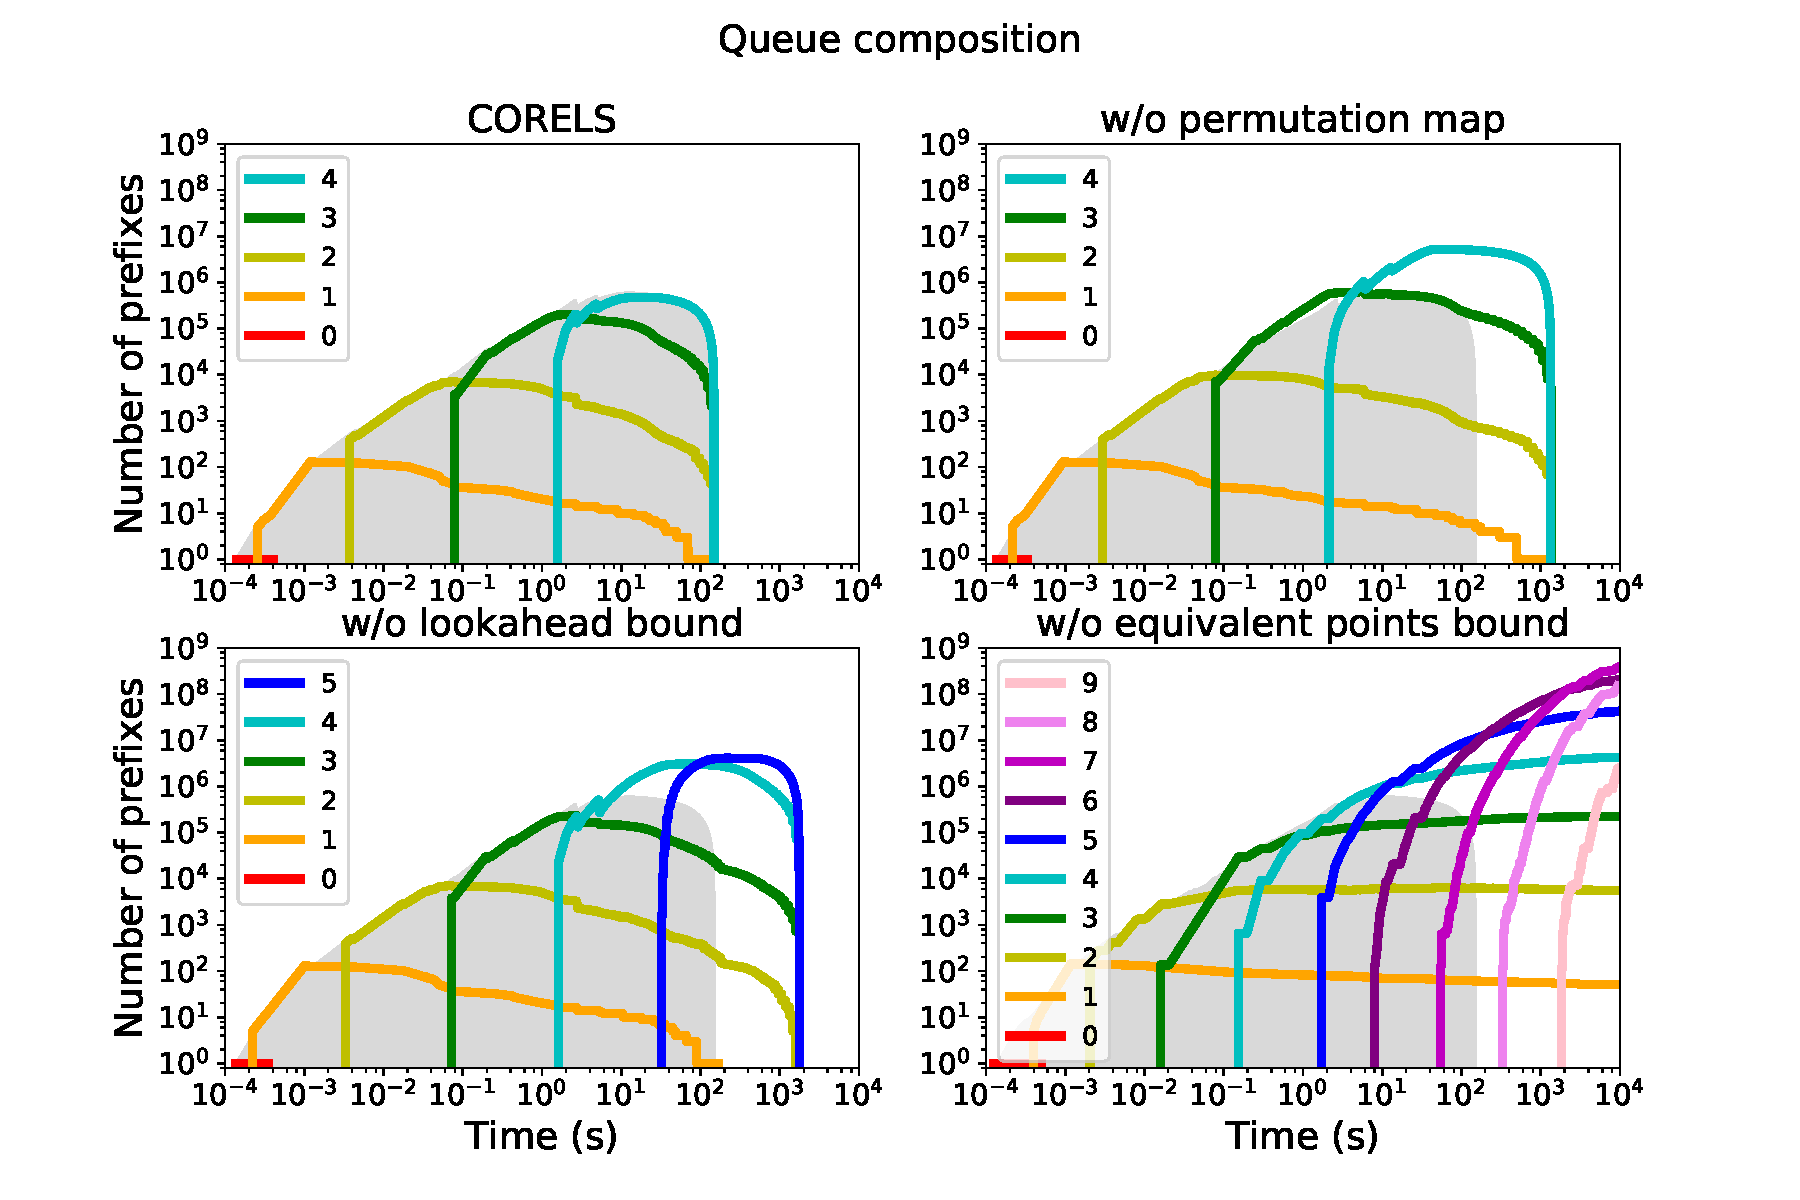
\includegraphics[trim={30mm 15mm 35mm 25mm}, width=0.45\textwidth]{figs/kdd_compas_compare_small-queue.pdf}
\end{kdd}
\end{center}
\caption{Queue composition. % logical queue
%
Numbers of prefixes in the queue (log scale), colored by length,
as a function of wall clock time (log scale),
for CORELS (top left), and without the permutation map (top right),
lookahead bound (bottom left), and equivalent points bound (bottom right).
%
The gray shading fills in the area beneath the total number of
queue elements for CORELS, \ie the sum over prefixes of lengths~0
through~4 in the top left figure.
%
For comparison, we replicate the same gray region
in the other three subfigures.
}
\label{fig:queue}
\end{figure}

%\begin{figure}[t!]
%\begin{center}
%%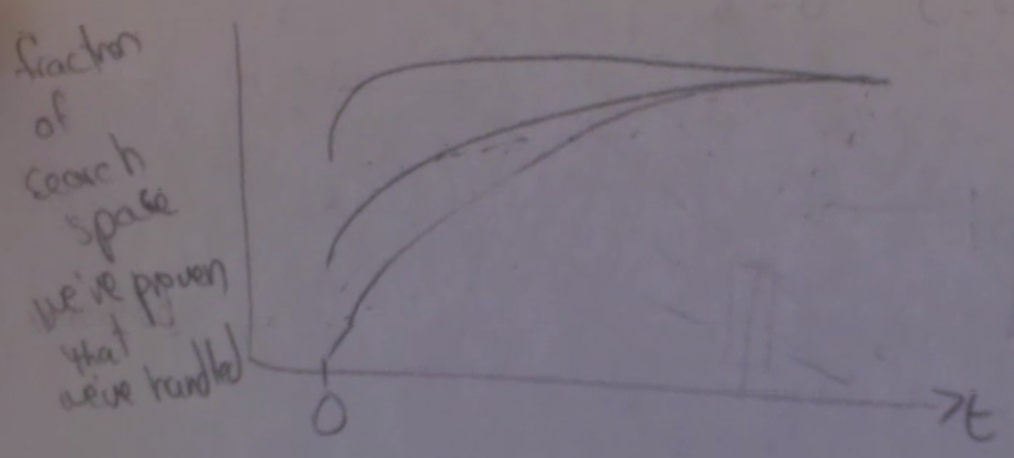
\includegraphics[width=0.65\textwidth]{figs/sketch-search-space.png}
%\begin{arxiv}
%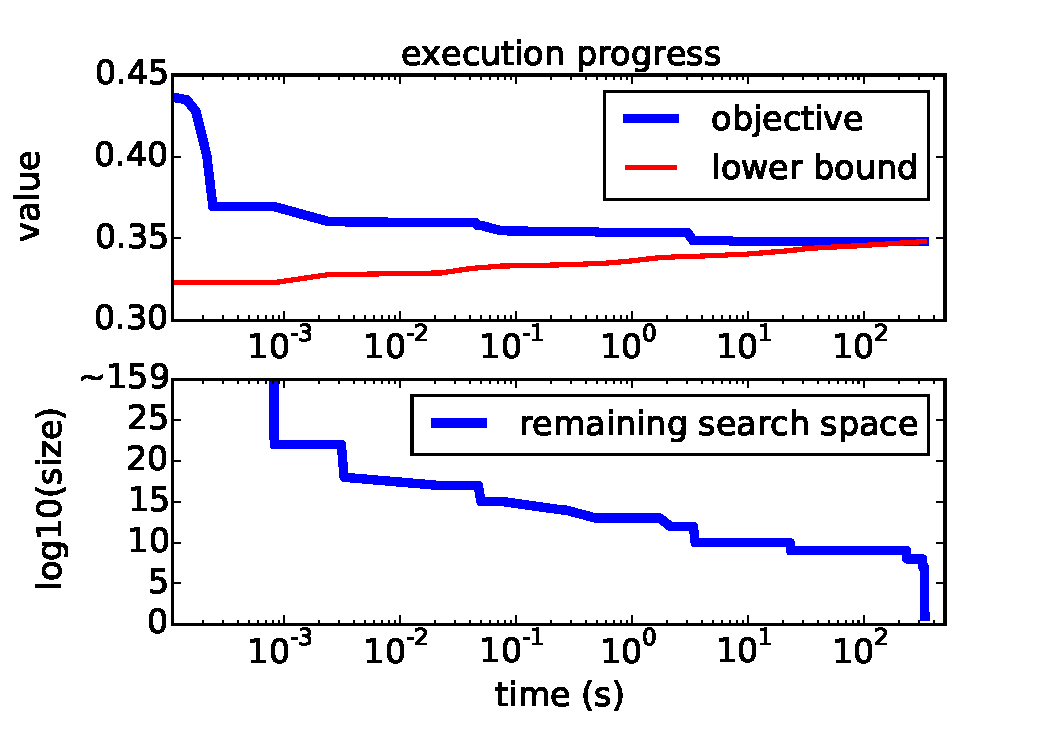
\includegraphics[width=0.8\textwidth]{figs/ela_compas-remaining-space.pdf}
%\end{arxiv}
%\begin{kdd}
%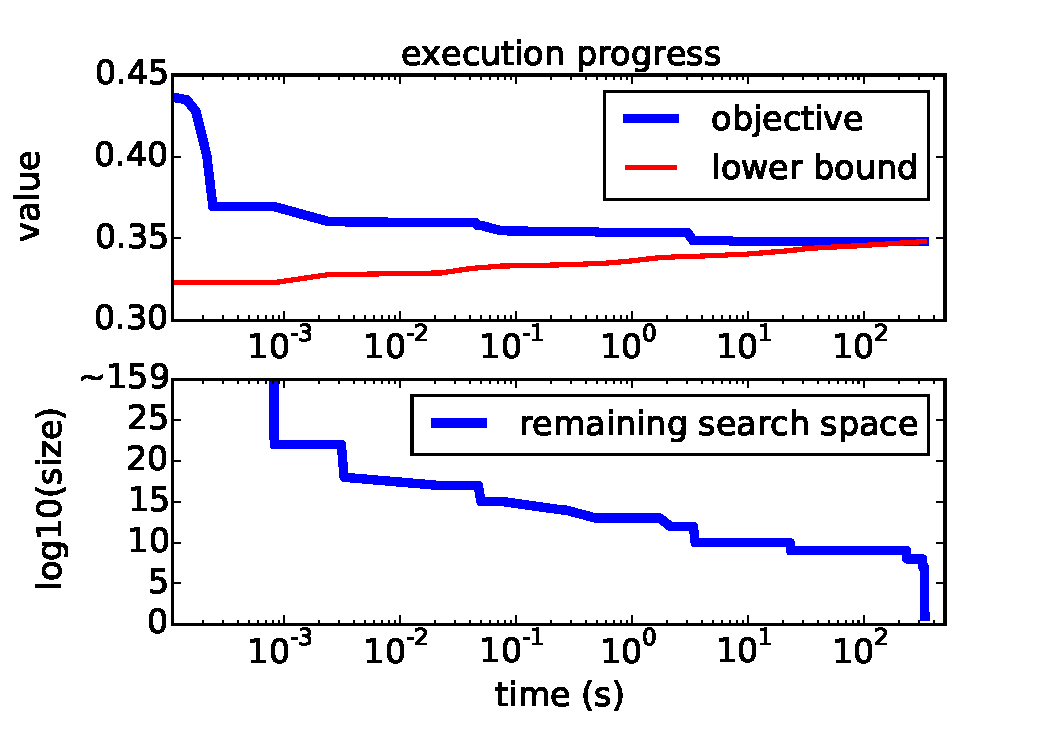
\includegraphics[width=0.5\textwidth]{figs/ela_compas-remaining-space.pdf}
%\end{kdd}
%\end{center}
%\caption{The logarithm (base 10) of the upper bound
%from Proposition~\ref{prop:remaining-eval-coarse}
%on the size of the remaining search space,
%as a function of wall clock time.
%%
%This bound depends on the total number of available rules,
%as well as two dynamic quantities:
%the current best objective value,
%and the histogram of logical queue elements,
%partitioned by prefix length.
%}
%\label{fig:search-space}
%\end{figure}

\begin{arxiv}
\begin{figure}[t!]
\begin{center}
%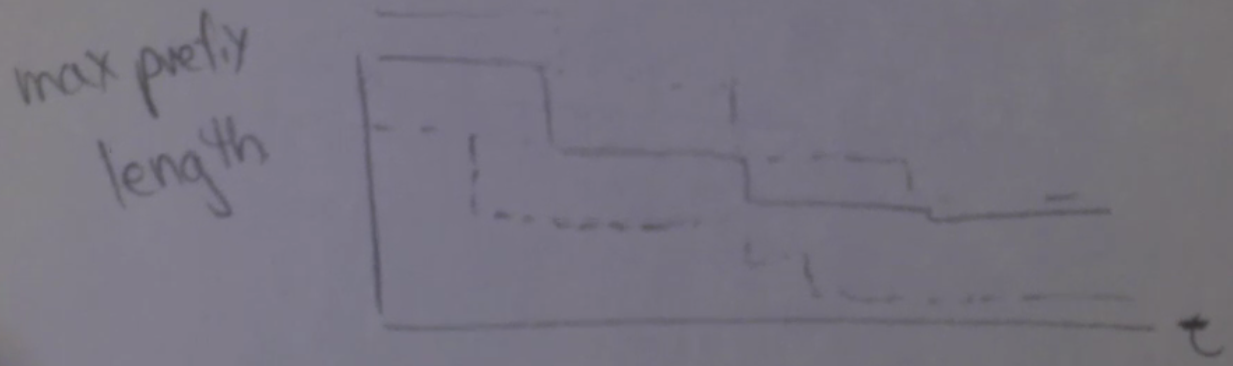
\includegraphics[width=0.65\textwidth]{figs/sketch-max-length.png}
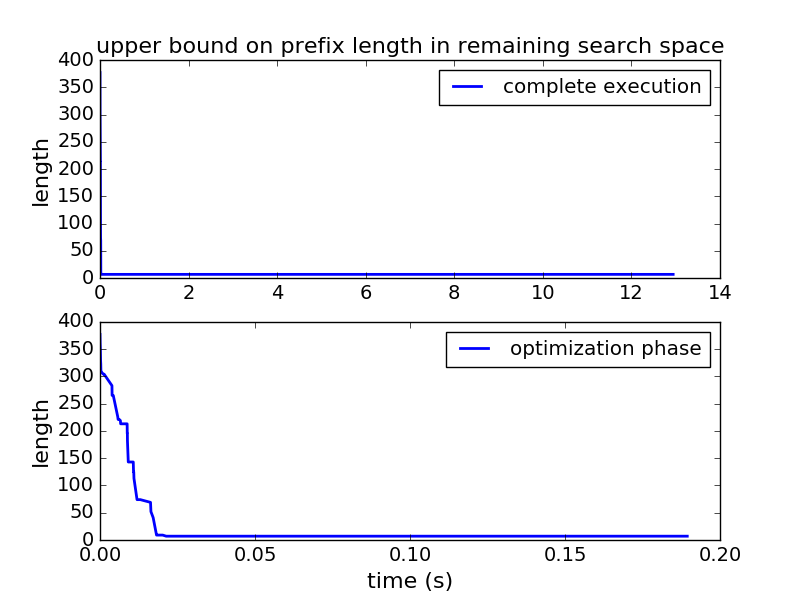
\includegraphics[width=0.8\textwidth]{figs/ela-max-length-check.png}
\end{center}
\caption{Max prefix length over time (computed from objective value)}
\label{fig:max-length}
\end{figure}

\begin{figure}[t!]
\begin{center}
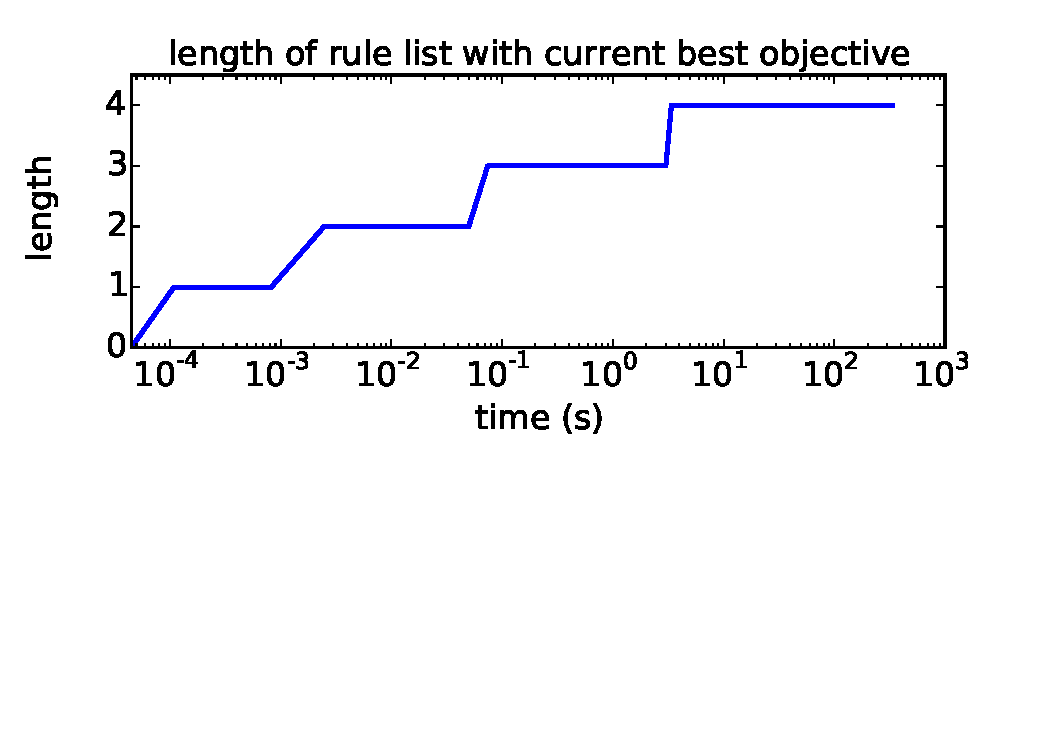
\includegraphics[width=0.8\textwidth]{figs/ela_compas-prefix-length.pdf}
\end{center}
\caption{Best prefix length over time}
\label{fig:prefix-length}
\end{figure}
\end{arxiv}
